\subsection{Combined Implementation}
\begin{figure}[H] 
	\centerline{
	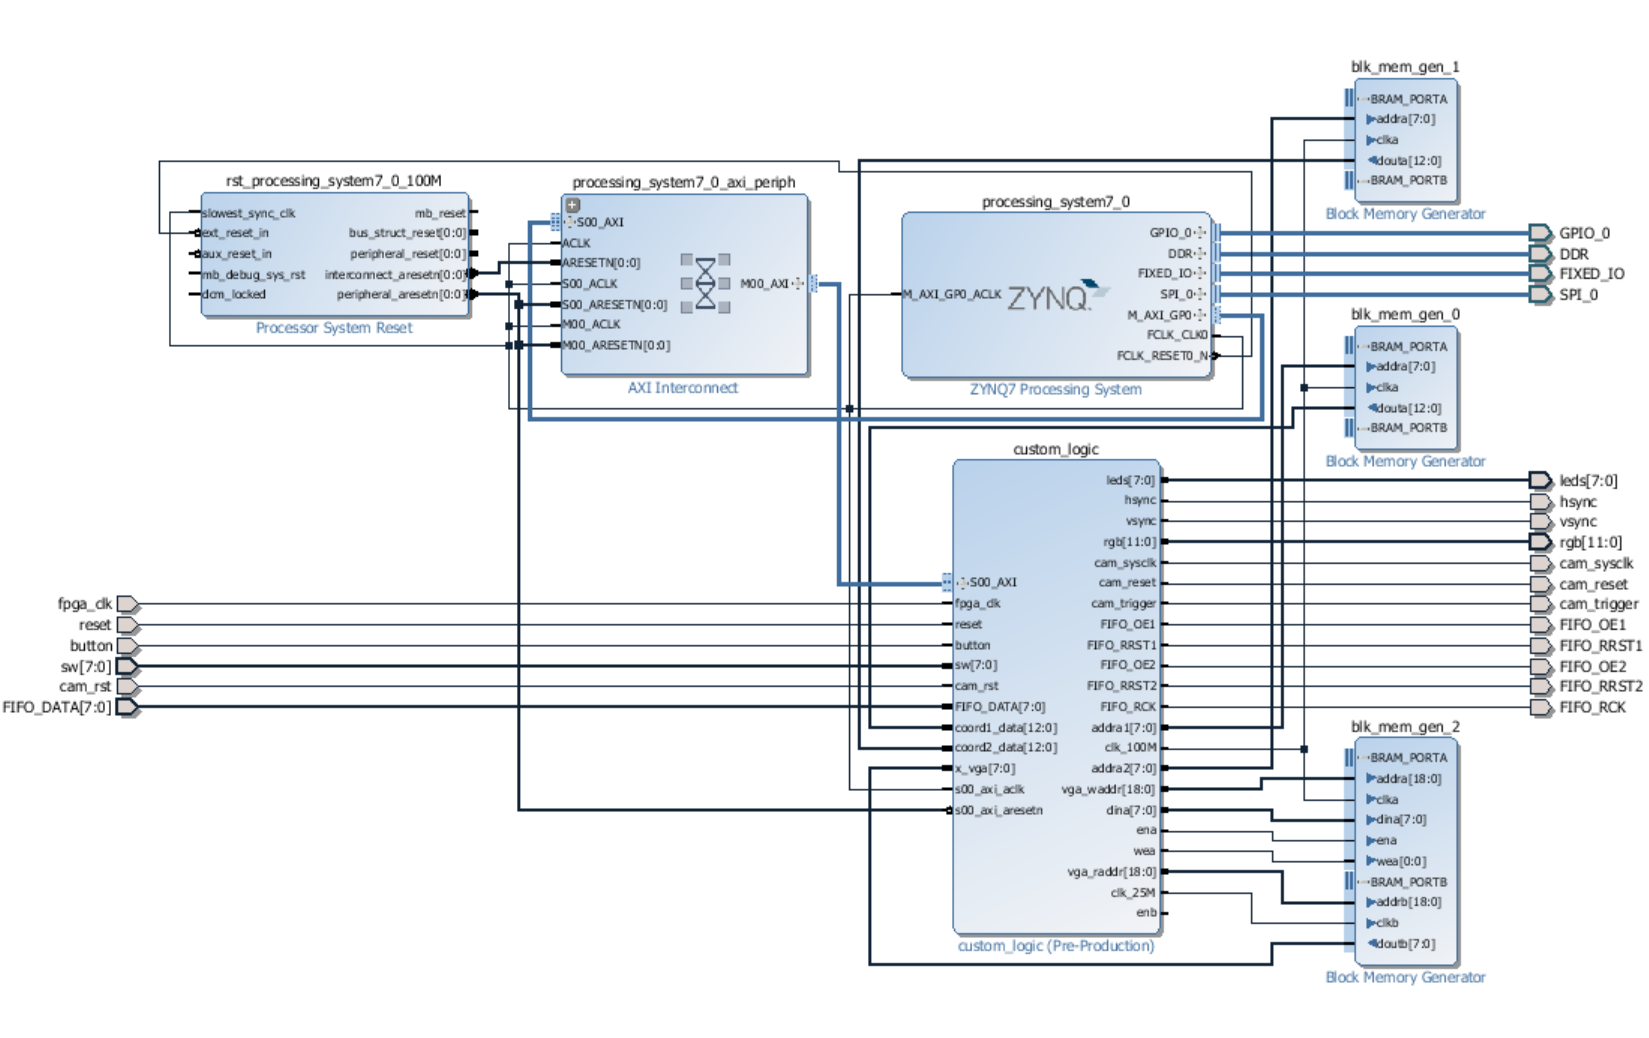
\includegraphics[width=1.25\linewidth, angle=90]{final_bd.png}
	}
	\caption{System Block Diagram}
	\label{finalBD}
\end{figure}

\begin{figure}[H] 
	\centerline{
	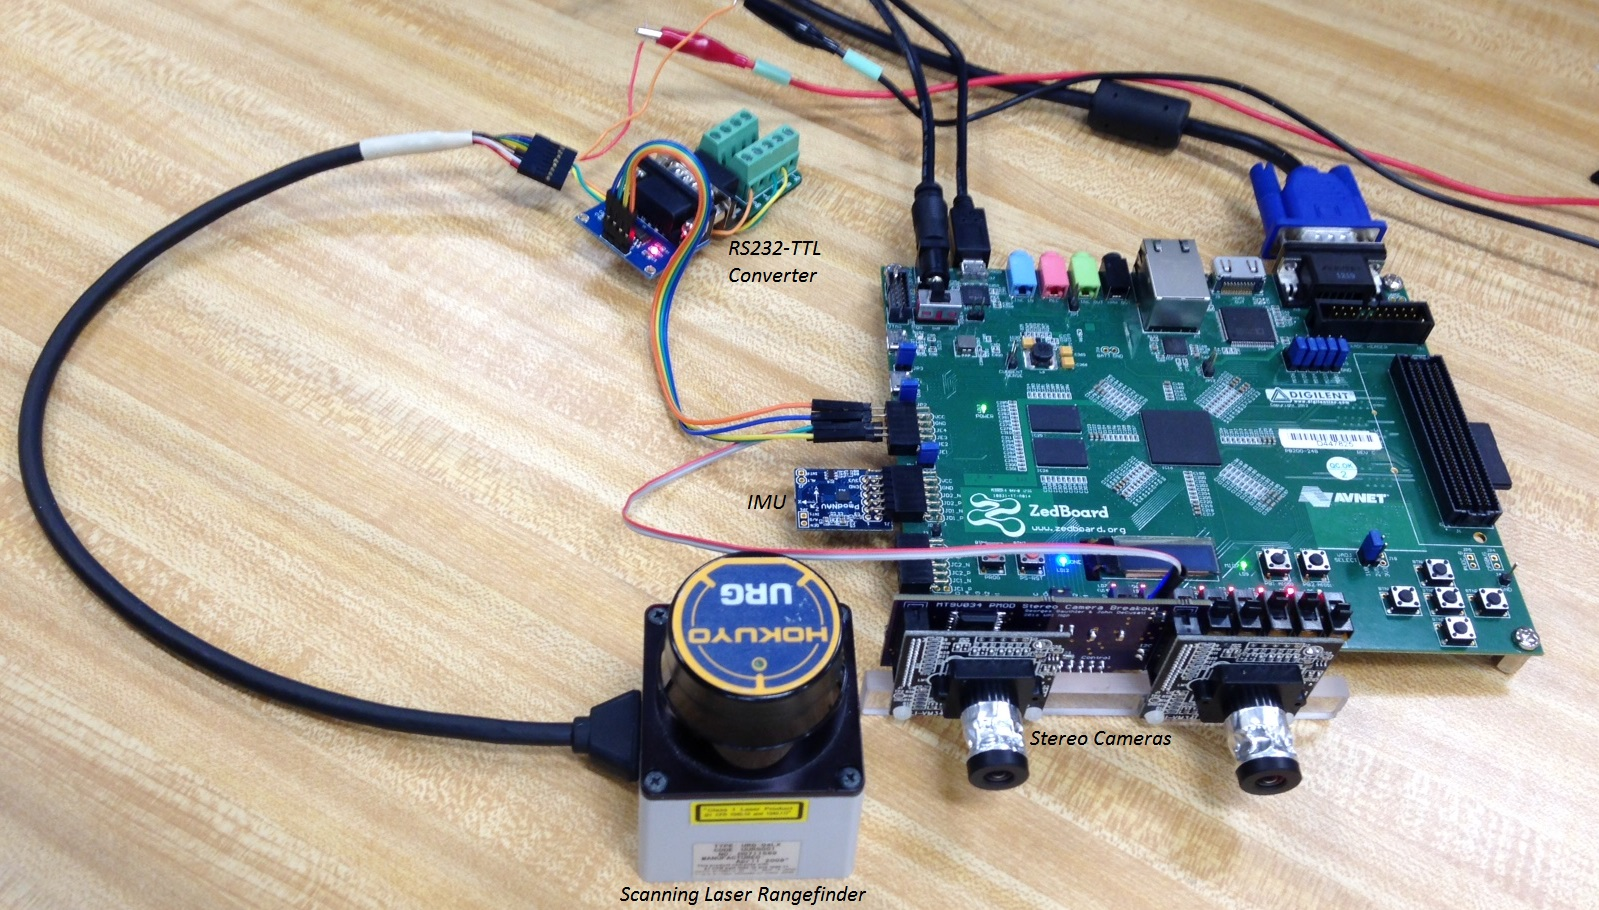
\includegraphics[width=0.85\linewidth]{setup.JPG}
	}
	\caption{System Hardware}
	\label{finalHW}
\end{figure}

\begin{figure}[H] 
         \begin{subfigure}[h]{0.5\textwidth}
              \centerline{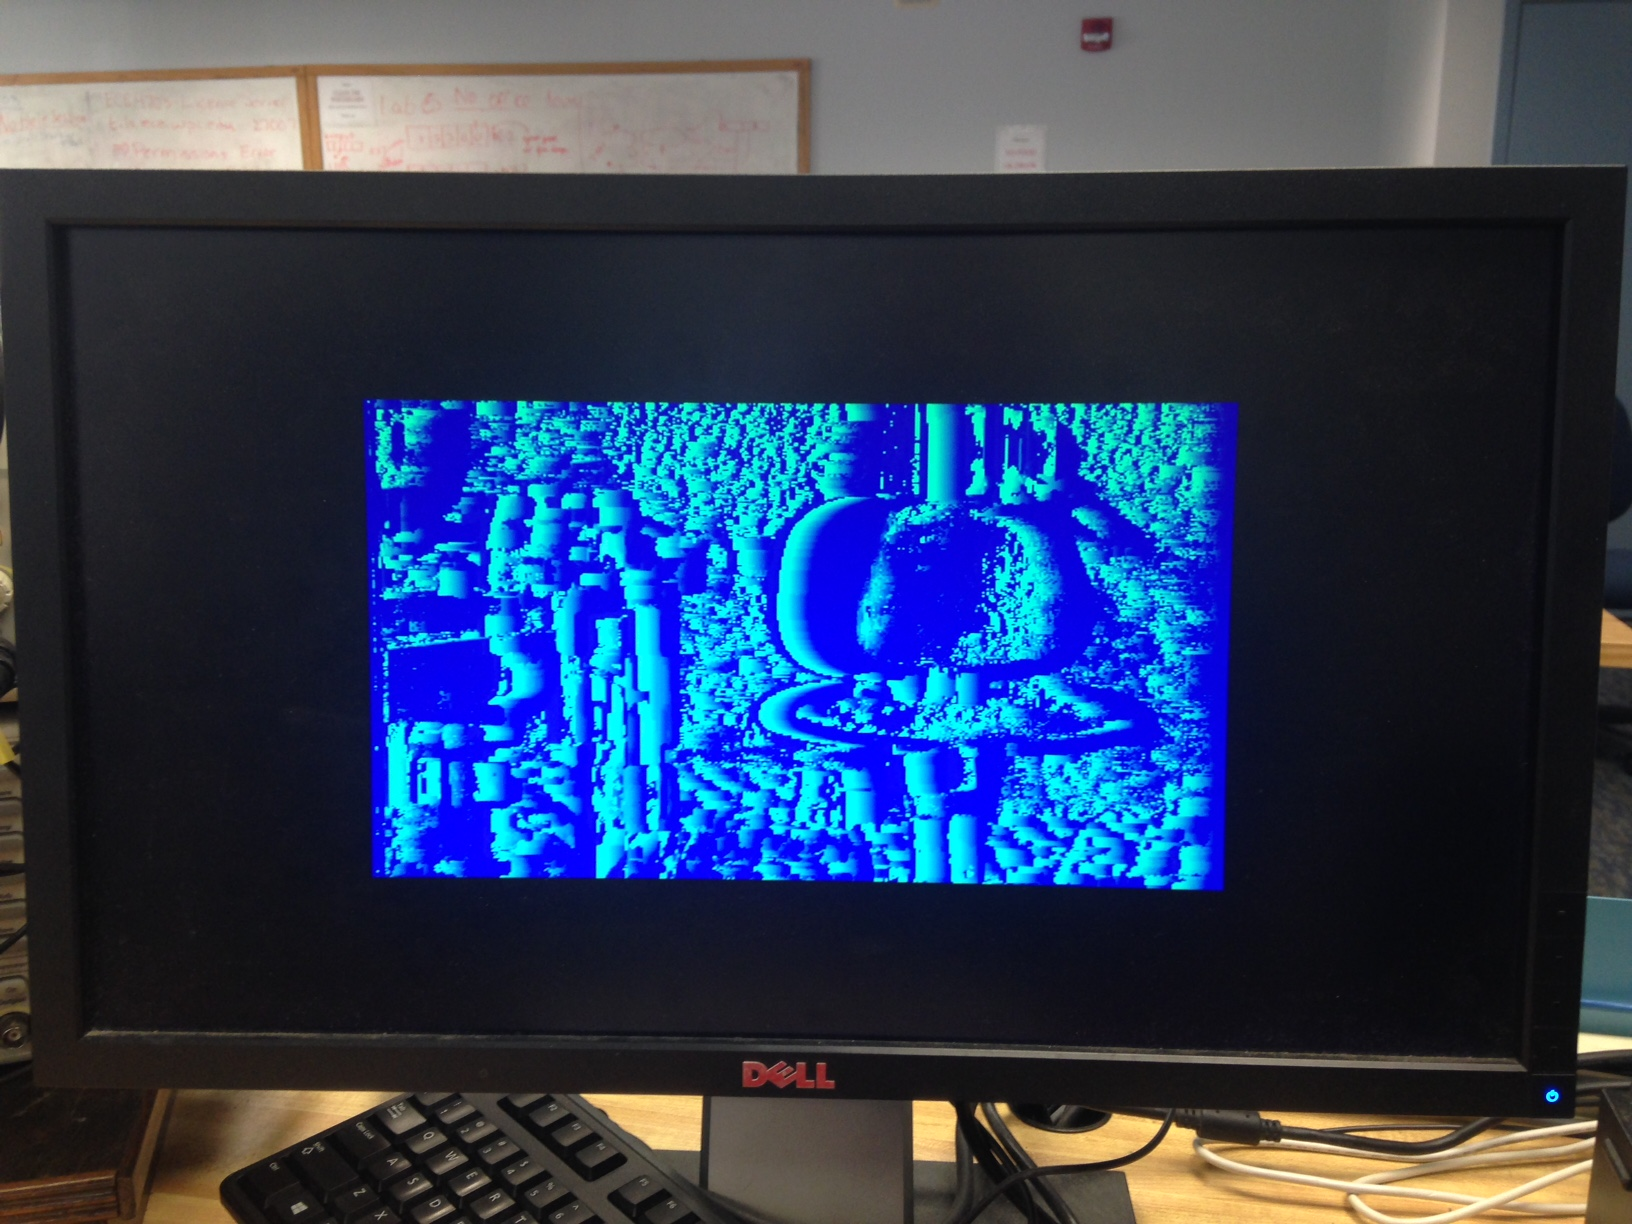
\includegraphics[width=1.0\textwidth]{disparity_mode.JPG}}
             \caption{Full Output}
         \end{subfigure}
         \begin{subfigure}[h]{0.5\textwidth}
             \centerline{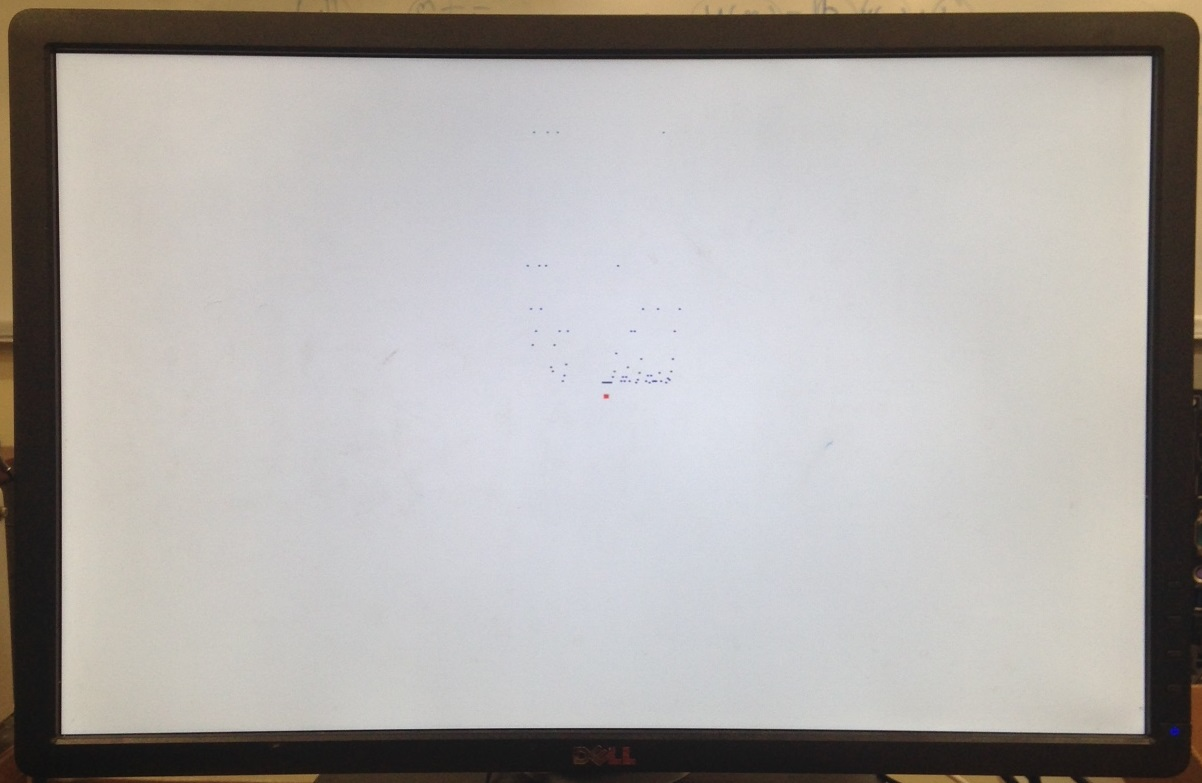
\includegraphics[width=1.0\textwidth]{disparity_line_mode.JPG}}
             \caption{Single Line Output}
         \end{subfigure}
\caption{Disparity Output Modes}
\label{disparityOutputs}
\end{figure}

\begin{figure}[H] 
         \begin{subfigure}[h]{0.5\textwidth}
              \centerline{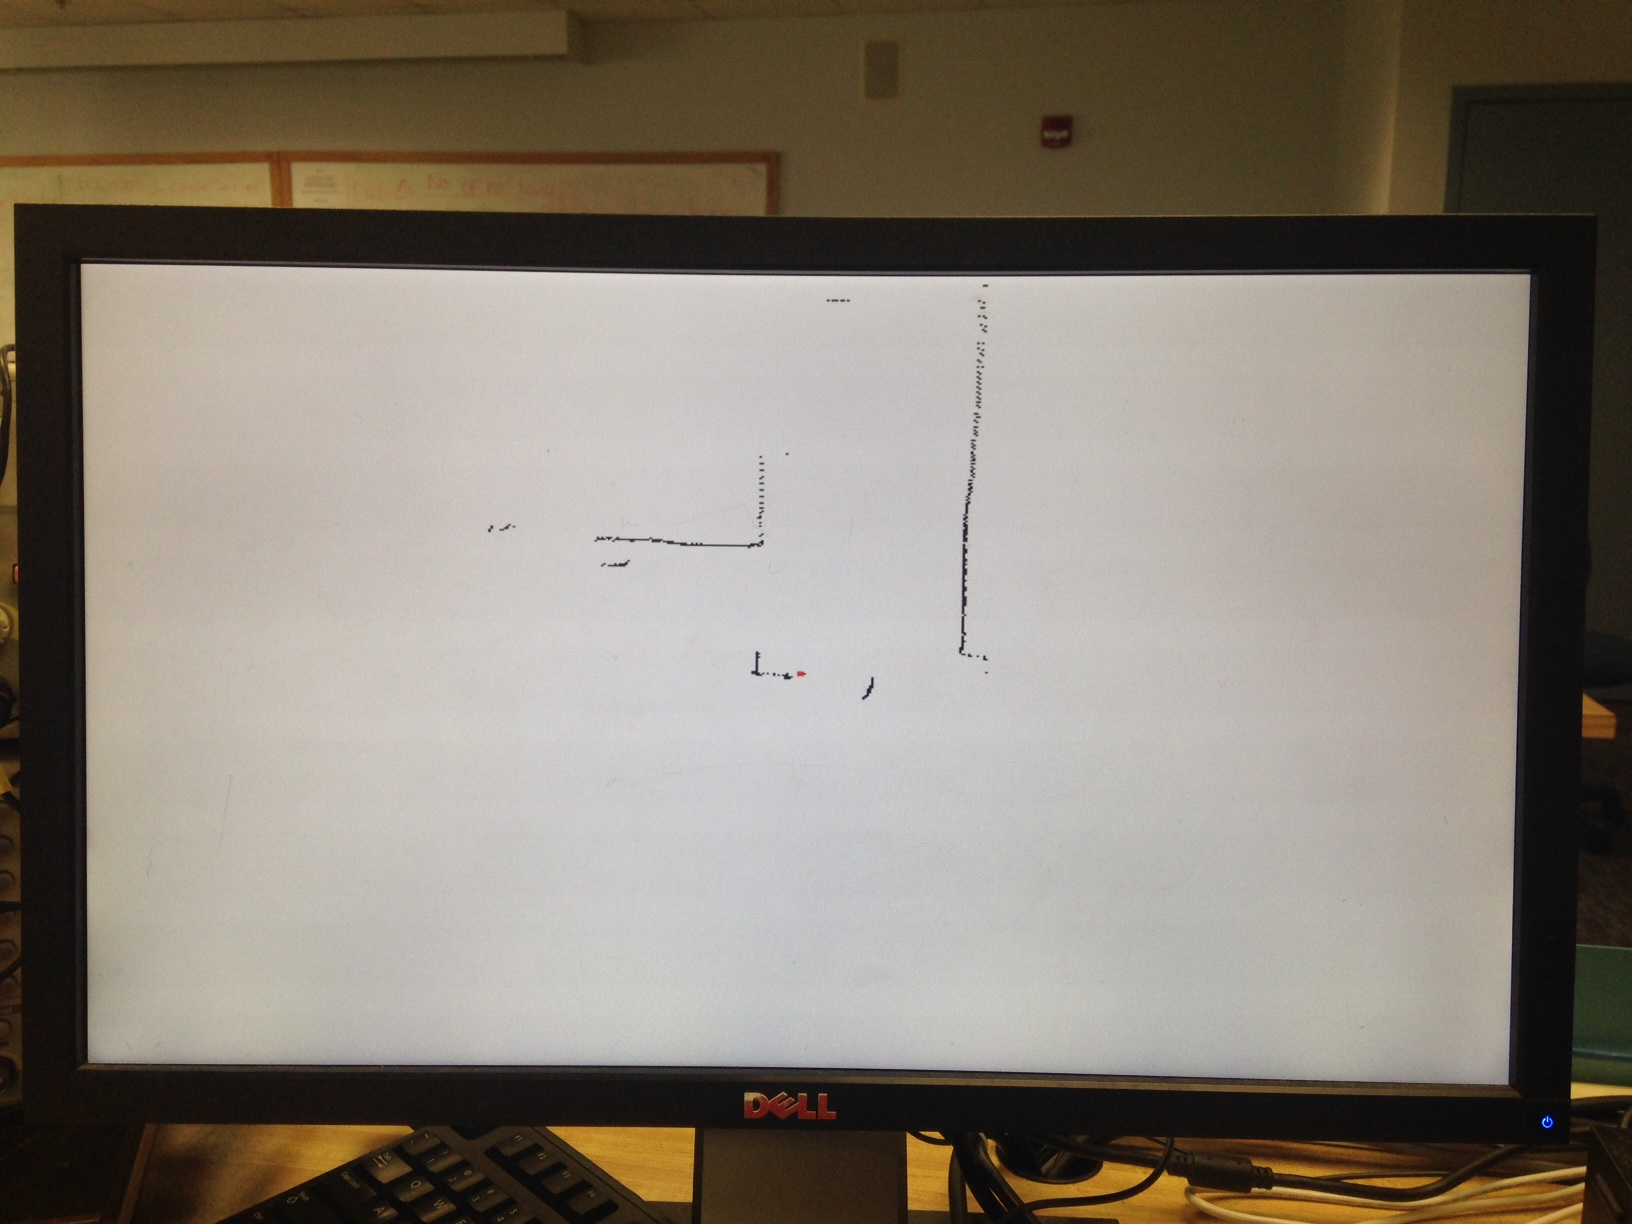
\includegraphics[width=1.0\textwidth]{rangefinder_mode.JPG}}
             \caption{Rangefinder Output}
         \end{subfigure}
         \begin{subfigure}[h]{0.5\textwidth}
             \centerline{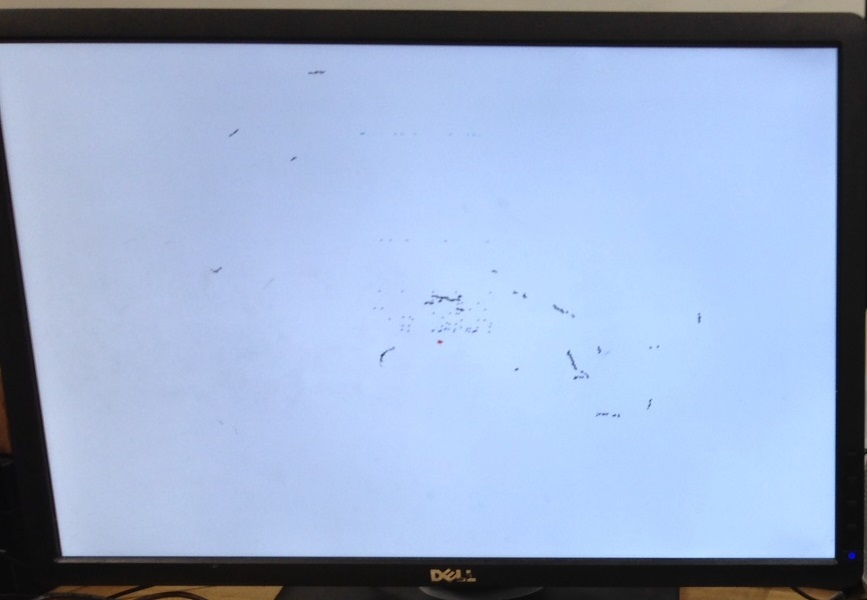
\includegraphics[width=1.0\textwidth]{combined_mode.JPG}}
             \caption{Combined Output}
         \end{subfigure}
\caption{2D "Floorplan" Output Modes}
\label{rangeOutputs}
\end{figure}
